\section{Introduction}
\label{sec:introduction}

\begin{figure}[t]
  \centering
  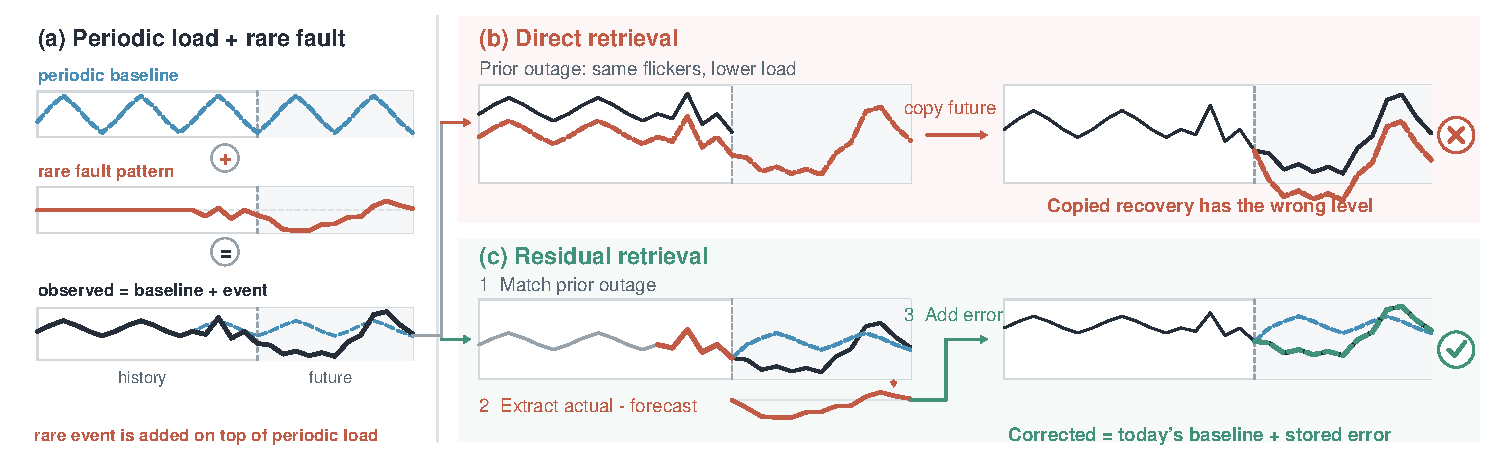
\includegraphics[width=\linewidth]{figures/intro_motivation.pdf}
  \caption{\textbf{Retrieve the error, not the input.} (a) An observed series is
  the sum of a dominant periodic component and an infrequent event. (b)
  Retrieving on the input matches a past window's \emph{routine} structure,
  which carries almost all of the window's energy; copying the future that
  followed then injects the old level and phase on top of a forecast that
  already had them right. (c) Subtracting the frozen forecaster's own prediction
  from that past outcome leaves only what it missed, turning the retrieved
  quantity into a correction that can be added to today's forecast.}
  \label{fig:motivation}
\end{figure}

Time-series forecasting supports decisions in electricity markets, traffic
management, and industrial operations, where the series mixes seasonality,
trend, abrupt change, and multiscale dependence
\citep{Chen2001FreewayPM,lago2021epf}. A decade of architectural work has
attacked this mixture through frequency decomposition, patching, cross-variable
attention, multiscale mixing, exogenous conditioning, and large-corpus
pretraining
\citep{zhou2022fedformer,patchtst,wu2023timesnet,liu2024itransformer,
wang2024timemixer,wang2024timexer,ansari2024chronos}. The resulting models are
strong at what they were designed for: they reproduce the routine level, phase,
and rhythm of a series with small average error.

What such a model gets wrong is therefore not the routine part of the signal.
The residual left after a trained forecaster has done its work is a small but
structured signal that concentrates on infrequent events, turning points, and
context-dependent biases, and that recurs whenever the generating condition
recurs. Retrieval exploits recurrence without touching a deployed model's
weights, and a growing family of retrieval-augmented forecasters does exactly
this
\citep{tire2024raf,zhang2024timeraf,han2025raft,ning2025tsrag}. Almost all of
them retrieve on the \emph{input}: they score historical windows by similarity
to the query context and reuse the futures that followed.
Figure~\ref{fig:motivation} shows why that object fits the error poorly.
Whole-window similarity is dominated by the periodic and trend structure the base
forecast already predicts, so the short prefix announcing a rare event rarely
decides which neighbours are returned; a well-matched neighbour's future still
carries its own level, phase, and covariate response, so transferring it
overwrites parts of the forecast that were already correct; and, beyond what the
figure shows, the retrieved neighbourhood is identical no matter which forecaster
is being augmented, so it cannot adapt to that forecaster's blind spot. Hence our
central question:

{\em When we augment a time-series forecaster with retrieval, what should we
retrieve?}

Our answer is \method{}, a post-hoc revision layer that retrieves a frozen
forecaster's \textbf{own past errors}. \method{} builds on the model-relative
decomposition $\ytrue = \ybase + \resid$, which splits a realized future into
what a specific forecaster predicted and what it missed. Rather than replacing
$\ybase$, \method{} keeps it as the query-specific prior and retrieves $\resid$
from a chronological memory of validation residuals whose targets were already
observable. Two choices make the retrieval model-adaptive: the query descriptor
is built from the observed context \emph{and} the forecaster's intended future,
so one window is described differently depending on what the model predicts for
it; and the memory stores that model's errors, so a different backbone retrieves
a different correction from the same data. Since retrieved errors help only when
errors recur, \method{} shrinks a correction whose neighbours disagree and
applies it only when held-out validation prefers it to simpler temporal and bias
corrections or to leaving the forecast untouched.

The design bears four advantages.
\textbf{(i) Model adaptivity:} index, stored targets, and correction are all
defined relative to one frozen forecaster, so \method{} adapts to its error
pattern instead of returning model-independent analogues.
\textbf{(ii) Post-hoc and model-agnostic:} \method{} consumes only predictions
and observed targets, never gradients or weights, so one interface covers neural
architectures, static ensembles, AutoML systems, and foundation models.
\textbf{(iii) Reliability awareness:} per-horizon, per-channel shrinkage and a
gate that can retain the untouched forecast make the recurring-error assumption
testable per deployment.
\textbf{(iv) Performance:} with every system revising identical frozen forecasts,
error retrieval improves all reported metrics in 490/585 settings and \method{}
in 533/585, against 375 and 384 for the published RAFT and SARAF operators.

Our contributions are threefold.
\textbf{(i) A shift of retrieval object:} we identify the retrieval object,
rather than the retrieval architecture, as the decision that determines whether
retrieval augmentation helps a trained forecaster, and argue for model-relative
errors over input windows and their futures.
\textbf{(ii) A practical algorithm:} \method{} turns that argument into a
reliability-aware, chronologically causal, validation-gated revision layer that
needs no retraining and no learned retriever.
\textbf{(iii) A systematic study:} we compare retrieval objects under a frozen
protocol with identical base forecasts, and measure the resulting layer across
13 architectures, six additional forecasting systems including AutoML and
foundation models, three published end-to-end retrieval systems, and a
forward-in-time prequential study.
